%package list
\documentclass{article}
\usepackage[top=3cm, bottom=3cm, outer=3cm, inner=3cm]{geometry}
\usepackage{multicol}
\usepackage{graphicx}
\usepackage{url}
\usepackage{graphicx}

%\usepackage{cite}
\usepackage{hyperref}
\usepackage{array}
%\usepackage{multicol}
\newcolumntype{x}[1]{>{\centering\arraybackslash\hspace{0pt}}p{#1}}
\usepackage{natbib}
\usepackage{pdfpages}
\usepackage{multirow}
\usepackage[normalem]{ulem}
\useunder{\uline}{\ul}{}
\usepackage{svg}
\usepackage{xcolor}
\usepackage{listings}
\lstdefinestyle{ascii-tree}{
    literate={├}{|}1 {─}{--}1 {└}{+}1 
  }
\lstset{basicstyle=\ttfamily,
  showstringspaces=false,
  commentstyle=\color{red},
  keywordstyle=\color{blue}
}
%\usepackage{booktabs}
\usepackage{caption}
\usepackage{subcaption}
\usepackage{float}
\usepackage{array}

\newcolumntype{M}[1]{>{\centering\arraybackslash}m{#1}}
\newcolumntype{N}{@{}m{0pt}@{}}


%%%%%%%%%%%%%%%%%%%%%%%%%%%%%%%%%%%%%%%%%%%%%%%%%%%%%%%%%%%%%%%%%%%%%%%%%%%%
%%%%%%%%%%%%%%%%%%%%%%%%%%%%%%%%%%%%%%%%%%%%%%%%%%%%%%%%%%%%%%%%%%%%%%%%%%%%

\newcommand{\itemStudent}{■Flores Nuñes, Rodrigo Francisco}
\newcommand{\itemStuden}{■Jimenez Paredes, Fabricio Gabriel}
\newcommand{\itemStude}{■Leon Ramos, Mijael Paul}
\newcommand{\itemStud}{■Paredes Miranda, Mauricio Antonio}
\newcommand{\itemCourseCode}{2025000}
\newcommand{\itemSemester}{I}
\newcommand{\itemUniversity}{Universidad Nacional de San Agustín de Arequipa}
\newcommand{\itemFaculty}{Facultad de Ingeniería de Producción y Servicios}
\newcommand{\itemDepartment}{Departamento Académico de Ingeniería de Sistemas e Informática}
\newcommand{\itemSchool}{Escuela Profesional de Ingeniería de Sistemas}
\newcommand{\itemAcademic}{2025 - A}
\newcommand{\itemInput}{Del 1 Julio 2025}
\newcommand{\itemOutput}{Al 27 Julio 2025}
\newcommand{\itemPracticeNumber}{01}
\newcommand{\itemTheme}{Sistema de control de versiones Git}
%%%%%%%%%%%%%%%%%%%%%%%%%%%%%%%%%%%%%%%%%%%%%%%%%%%%%%%%%%%%%%%%%%%%%%%%%%%%
%%%%%%%%%%%%%%%%%%%%%%%%%%%%%%%%%%%%%%%%%%%%%%%%%%%%%%%%%%%%%%%%%%%%%%%%%%%%

\usepackage[english,spanish]{babel}
\usepackage[utf8]{inputenc}
\AtBeginDocument{\selectlanguage{spanish}}
\renewcommand{\figurename}{Figura}
\renewcommand{\refname}{Referencias}
\renewcommand{\tablename}{Tabla} %esto no funciona cuando se usa babel
\AtBeginDocument{%
	\renewcommand\tablename{Tabla}
}

\usepackage{fancyhdr}
\pagestyle{fancy}
\fancyhf{}
\setlength{\headheight}{40.51407pt}
\renewcommand{\headrulewidth}{1pt}
\renewcommand{\footrulewidth}{1pt}
\fancyhead[L]{\raisebox{-0.2\height}{
\includegraphics[width=3cm]{img/logo_episunsa.png}}}
\fancyhead[C]{\fontsize{7}{7}\selectfont	\itemUniversity \\ \itemFaculty \\ \itemDepartment \\ \itemSchool \\ \textbf{\itemCourse}}
\fancyhead[R]{\raisebox{-0.2\height}{
\includegraphics[width=1.2cm]{img/logo_abet}}}
\fancyfoot[L]{ESGames}
\fancyfoot[C]{\itemCourse}
\fancyfoot[R]{Página \thepage}

% para el codigo fuente
\usepackage{listings}
\usepackage{color, colortbl}
\definecolor{dkgreen}{rgb}{0,0.6,0}
\definecolor{gray}{rgb}{0.5,0.5,0.5}
\definecolor{mauve}{rgb}{0.58,0,0.82}
\definecolor{codebackground}{rgb}{0.95, 0.95, 0.92}
\definecolor{tablebackground}{rgb}{0.8, 0, 0}

\lstset{frame=tb,
	language=bash,
	aboveskip=3mm,
	belowskip=3mm,
	showstringspaces=false,
	columns=flexible,
	basicstyle={\small\ttfamily},
	numbers=none,
	numberstyle=\tiny\color{gray},
	keywordstyle=\color{blue},
	commentstyle=\color{dkgreen},
	stringstyle=\color{mauve},
	breaklines=true,
	breakatwhitespace=true,
	tabsize=3,
	backgroundcolor= \color{codebackground},
}

\begin{document}
	
	\vspace*{10px}
	
	\begin{center}	
		\fontsize{17}{17} \textbf{ PROYECTO FINAL }
	\end{center}
	\centerline{\textbf{ESGames: Desarrollo de una Plataforma Web para la Venta de Videojuegos Utilizando \\ Django y Vue.js}}
	%\vspace*{0.5cm}	


	\begin{table}[h!]
		\begin{tabular}{|x{4.7cm}|x{4.8cm}|x{4.8cm}|}        
			\hline 
			\rowcolor{tablebackground}
			\color{white} \textbf{Estudiantes} & \color{white}\textbf{Escuela}  & \color{white}\textbf{Asignatura}   \\
			\hline 
			{\itemStudent \par \itemStuden \par \itemStude \par \itemStud} & \itemSchool & {Programación Web II \par Semestre: III  }\\
			\hline 			
		\end{tabular}
	\end{table}		
	

	
	\begin{table}[H]
		\begin{tabular}{|x{4.7cm}|x{4.8cm}|x{4.8cm}|}
			\hline 
			\rowcolor{tablebackground}
			\color{white}\textbf{Semestre académico} & \color{white}\textbf{Fecha de inicio}  & \color{white}\textbf{Fecha de entrega}   \\
			\hline 
			\itemAcademic & \itemInput &  \itemOutput  \\
			\hline 
		\end{tabular}
	\end{table}
	
	\section{Tipo de Sistema}

ESGames es una aplicación web de comercio digital que simula una tienda virtual de videojuegos, desarrollada con el framework Django 4 para el backend y Vue.js para el frontend. La arquitectura adoptada se basa en el modelo cliente-servidor, con una API RESTful que permite el intercambio eficiente de información entre ambos extremos de la aplicación. La interfaz de usuario (frontend) fue construida como una Single Page Application (SPA) y desplegada en Netlify, una plataforma especializada en alojamiento de sitios estáticos y aplicaciones web modernas. El backend fue desplegado en Render, un servicio en la nube que permite alojar aplicaciones web y APIs, ofreciendo soporte nativo para proyectos Django y PostgreSQL.

		
\section{Modelo de Datos}

El sistema \textbf{ESGames} implementa un modelo de datos relacional basado en una arquitectura cliente-servidor. Las entidades se definieron inicialmente en Django ORM y posteriormente se adaptaron para su implementación en Supabase. A continuación, se describen las entidades principales y sus relaciones.

\subsection{Entidades Principales}

\begin{itemize}
  \item \textbf{UserProfile}: Representa a un usuario registrado. Se relaciona uno a uno con el modelo \texttt{User} de Django. Puede tener un carrito de compras, múltiples videojuegos adquiridos, favoritos y valoraciones.
  
  \item \textbf{Videogame}: Representa un videojuego en la tienda. Contiene información como título, descripción, precio, fecha de lanzamiento y pertenece a una categoría. Puede estar relacionado con muchos carritos, bibliotecas, favoritos y reseñas.
  
  \item \textbf{Cart}: Representa el carrito de compras de un usuario. Se relaciona uno a uno con un \texttt{UserProfile} y contiene múltiples \texttt{CartItem}.
  
  \item \textbf{CartItem}: Representa un ítem dentro del carrito de compras. Se asocia a un carrito y a un videojuego específicos.
  
  \item \textbf{Library}: Representa los videojuegos adquiridos por un usuario. Permite establecer una relación de muchos a muchos entre usuarios y videojuegos, almacenando además la fecha de adquisición.
  
  \item \textbf{Favorite}: Representa los videojuegos marcados como favoritos por un usuario. Establece una relación muchos a muchos entre \texttt{UserProfile} y \texttt{Videogame}.
  
  \item \textbf{Review}: Representa una reseña escrita por un usuario para un videojuego adquirido. Contiene un comentario, una calificación de 1 a 5 y la fecha de emisión.
\end{itemize}

\subsection{Relaciones entre Entidades}

\begin{itemize}
  \item Un \texttt{UserProfile} tiene:
  \begin{itemize}
    \item Un \texttt{Cart} (relación 1:1).
    \item Muchos \texttt{CartItem} a través del \texttt{Cart}.
    \item Muchos \texttt{Library}, \texttt{Favorite} y \texttt{Review}.
  \end{itemize}
  
  \item Un \texttt{Videogame} puede:
  \begin{itemize}
    \item Estar en múltiples \texttt{CartItem}, \texttt{Library}, \texttt{Favorite} y \texttt{Review}.
    \item Pertenecer a una \texttt{Category}.
  \end{itemize}
  
  \item Un \texttt{Cart} tiene muchos \texttt{CartItem}.
  
  \item Un \texttt{Library} y un \texttt{Favorite} representan relaciones N:M entre \texttt{UserProfile} y \texttt{Videogame}.
\end{itemize}

\subsection{Modelo Relacional}

A continuación se muestra un resumen simplificado de las relaciones:

\begin{itemize}
  \item \texttt{UserProfile} $\longrightarrow$ \texttt{Cart} (1:1)
  \item \texttt{Cart} $\longrightarrow$ \texttt{CartItem} (1:N)
  \item \texttt{CartItem} $\longrightarrow$ \texttt{Videogame} (N:1)
  \item \texttt{UserProfile} $\longrightarrow$ \texttt{Library} $\longleftarrow$ \texttt{Videogame} (N:M)
  \item \texttt{UserProfile} $\longrightarrow$ \texttt{Favorite} $\longleftarrow$ \texttt{Videogame} (N:M)
  \item \texttt{UserProfile} $\longrightarrow$ \texttt{Review} $\longleftarrow$ \texttt{Videogame} (1:N)
  \item \texttt{Videogame} $\longrightarrow$ \texttt{Category} (N:1)
\end{itemize}


	
\section{Diccionario de Datos: \texttt{Videogame}}
La tabla Videogame es una de las entidades centrales del sistema ESGames, ya que representa el producto principal que los usuarios pueden explorar, comprar, valorar o marcar como favorito. Su diseño busca ser lo suficientemente flexible para almacenar tanto los datos descriptivos como las referencias necesarias para integrarse con otras entidades del sistema.
\begin{table}[H]
\centering
\begin{tabular}{|l|l|c|c|l|p{6cm}|}
\hline
\textbf{Atributo} & \textbf{Tipo} & \textbf{Nulo} & \textbf{Clave} & \textbf{Predeterminado} & \textbf{Descripción} \\
\hline
id & Entero & No & Primaria & Autoincremental & Identificador único del videojuego. \\
title & Cadena (50) & No & No & Ninguno & Título del videojuego. \\
description & Texto & Sí & No & Vacío & Descripción del contenido del videojuego. \\
price & Decimal(10,2) & No & No & Ninguno & Precio del Videojuego. \\
stock & Entero & No & No & 0 & Cantidad disponible para comprar. \\
release\_date & Fecha & Sí & No & NULL & Fecha de lanzamiento oficial del videojuego. \\
category\_id & Entero (FK) & Sí & Foránea & NULL & Categoría a la que pertenece el videojuego. \\
image\_url & Cadena (255) & Sí & No & Vacío & URL de la imagen del videojuego. \\
\hline
\end{tabular}
\caption{Diccionario de datos de la entidad \texttt{Videogame}.}
\end{table}

\section{Diagrama Entidad-Relación}
El siguiente diagrama representa las entidades principales del sistema \textbf{ESGames} y sus relaciones. Cada entidad contiene atributos relevantes para el funcionamiento del sistema, y las relaciones reflejan cómo interactúan los usuarios con los videojuegos mediante compras, favoritos, valoraciones y carrito de compras.

\begin{figure}[H]
    \centering
    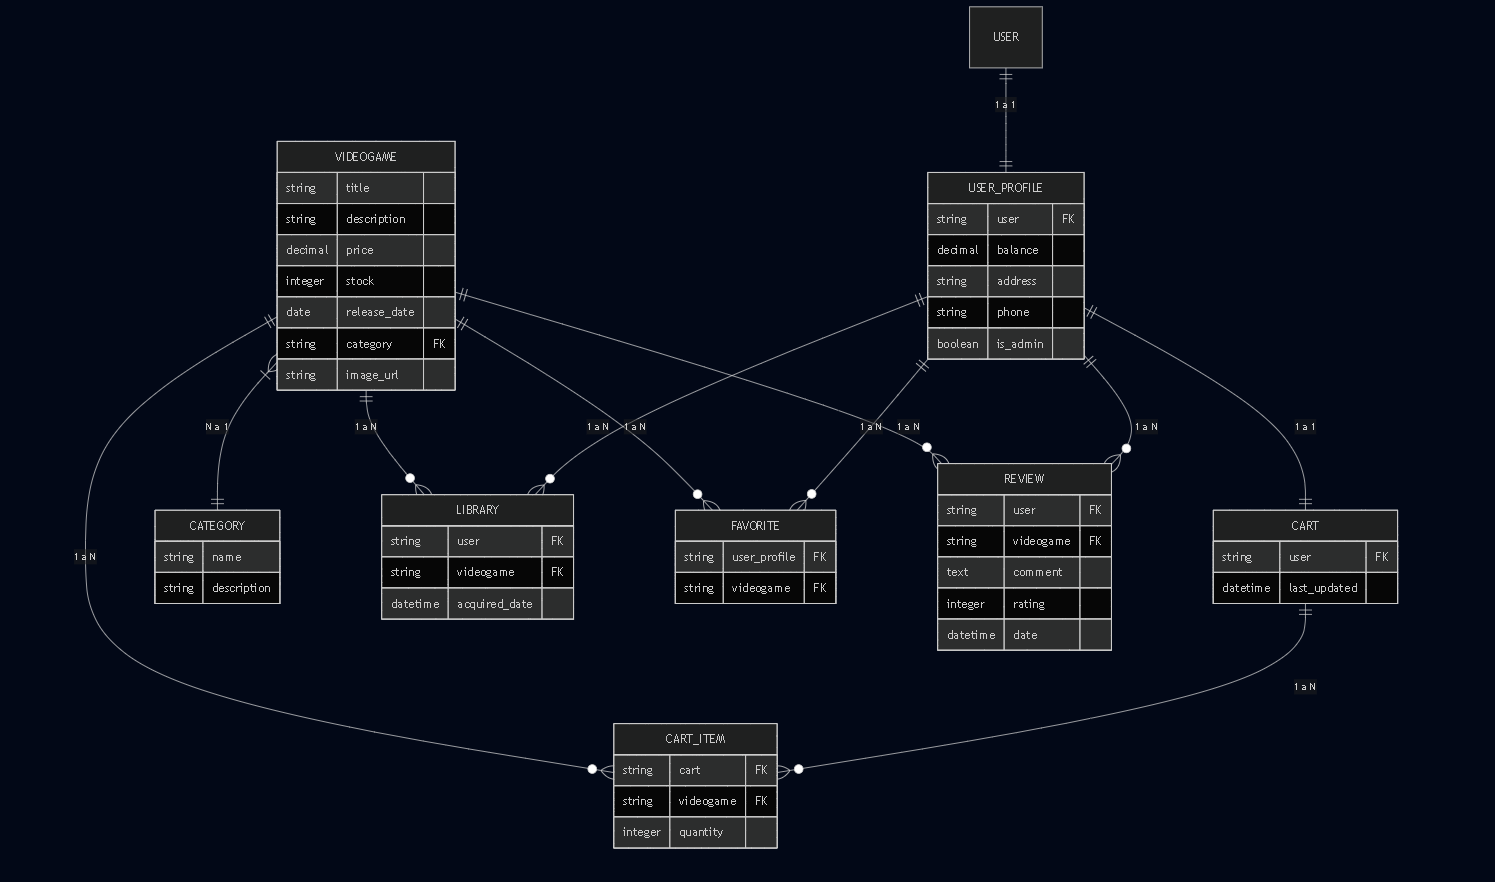
\includegraphics[width=0.9\linewidth]{img/datos2.png}
    \caption{Diagrama Entidad-Relación del sistema \texttt{ESGames}.}
\end{figure}

	

\section{Administración con Django}

Para la implementación del sistema \textbf{ESGames}, se utilizó el framework \texttt{Django 4}, el cual proporciona un sistema administrativo robusto para gestionar modelos y datos de forma eficiente. A continuación, se describen los pasos realizados para configurar la administración y gestión del sistema:

\subsection{Creación del Proyecto y la Aplicación}

Se inició la construcción del sistema mediante los siguientes comandos:

\begin{verbatim}
django-admin startproject gameStore
cd gameStore
python manage.py startapp ESGames
\end{verbatim}

El proyecto principal \texttt{gameStore} contiene la configuración global del sistema, mientras que la aplicación \texttt{ESGames} encapsula los modelos, vistas, serializadores y lógica de negocio principal.

\subsection{Definición de Modelos}

Los modelos del sistema, como \texttt{Videogame}, \texttt{UserProfile}, \texttt{Cart}, \texttt{CartItem}, entre otros, fueron definidos en la carpeta \texttt{models/.py}, utilizando el ORM de Django. Cada modelo representa una tabla en la base de datos relacional.

\subsection{Generación y Aplicación de Migraciones}

Una vez definidos los modelos, se generaron las migraciones necesarias para sincronizar la base de datos mediante:

\begin{verbatim}
python manage.py makemigrations
python manage.py migrate
\end{verbatim}

Esto permitió crear las estructuras de tablas en Supabase, la base de datos relacional utilizada por el sistema.

\subsection{Habilitación del Panel de Administración}

Django proporciona una interfaz administrativa integrada en la URL \texttt{/admin}. Para habilitar el acceso, se registraron los modelos en el archivo \texttt{ESGames/admin.py}:

\begin{verbatim}
from django.contrib import admin
from .models import Videogame, UserProfile, Cart, CartItem, Review, Favorite, Library

admin.site.register(Videogame)
admin.site.register(UserProfile)
admin.site.register(Cart)
admin.site.register(CartItem)
admin.site.register(Review)
admin.site.register(Favorite)
admin.site.register(Library)
\end{verbatim}

\subsection{Creación de Superusuario}

Para acceder al panel de administración, se creó un superusuario ejecutando:

\begin{verbatim}
python manage.py createsuperuser
\end{verbatim}

Una vez autenticado, se pudo gestionar videojuegos, usuarios, reseñas y otros datos del sistema directamente desde el panel administrativo web.

\subsection{Ventajas del Administrador de Django}

El sistema administrativo permitió:

\begin{itemize}
  \item Visualización y edición de registros sin necesidad de crear interfaces personalizadas.
  \item Creación, modificación y eliminación de datos relacionados con usuarios y productos.
  \item Validación automática de formularios.
  \item Control de acceso mediante credenciales y permisos.
\end{itemize}

Este entorno aceleró significativamente el proceso de pruebas y carga de información durante el desarrollo.



\section{Estructura del Frontend}

El frontend del sistema \textbf{ESGames} fue desarrollado utilizando el framework \texttt{Vue.js 3} en conjunto con \texttt{Vite} como sistema de empaquetado. El despliegue del cliente se realizó en la plataforma \texttt{Netlify}, lo cual permite una integración continua y despliegue automático tras cada cambio en el repositorio.

\subsection{Organización del Proyecto}

La estructura del proyecto está organizada de forma modular en la carpeta \texttt{src}, la cual contiene los siguientes elementos principales:

\begin{itemize}
    \item \textbf{views/}: Contiene las vistas principales del sistema como Home, Login, Register, Store, Cart y GameDetails.
    \item \textbf{components/}: Aquí se encuentran los componentes reutilizables como tarjetas de videojuegos, encabezados, formularios, etc.
    \item \textbf{api/}: Funciones centralizadas que gestionan la comunicación con el backend desplegado en Render.
    \item \textbf{router/}: Configuración de rutas mediante \texttt{vue-router}, definiendo navegación entre vistas.
    \item \textbf{store/}: Gestión de estado global usando \texttt{Pinia}, permitiendo mantener sincronizados los datos del usuario, carrito y biblioteca.
    \item \textbf{style.css}: Archivo global de estilos con diseño personalizado inspirado en estética moderna de videojuegos.
\end{itemize}

\subsection{Diseño Visual y Experiencia de Usuario}

El diseño visual fue desarrollado de forma personalizada mediante hojas de estilo CSS y aprovechando clases utilitarias. El estilo general busca una interfaz amigable, clara y responsiva, con una paleta de colores oscura y elementos destacados mediante efectos sutiles como sombras y bordes redondeados.

\subsection{Navegación y Responsividad}

Se implementó un sistema de rutas dinámicas que permite cargar detalles de cada videojuego desde la API del backend. El sistema es responsivo, adaptándose a dispositivos móviles y pantallas de escritorio gracias al uso de Flexbox y media queries.

\subsection{Ventajas del Enfoque Modular}

El uso de Vue.js y la separación de vistas y componentes favorece la mantenibilidad, la escalabilidad y la reutilización de código. Esto permite futuras mejoras en el diseño o integración de nuevas funcionalidades sin alterar el núcleo del sistema.

\subsection{Despliegue}

El proyecto fue desplegado en \texttt{Netlify}, aprovechando su integración con GitHub y su soporte para proyectos Vite. Cada vez que se hace un \texttt{push} a la rama principal, el sistema se vuelve a compilar y actualizar automáticamente.
\begin{figure}[H]
    \centering
    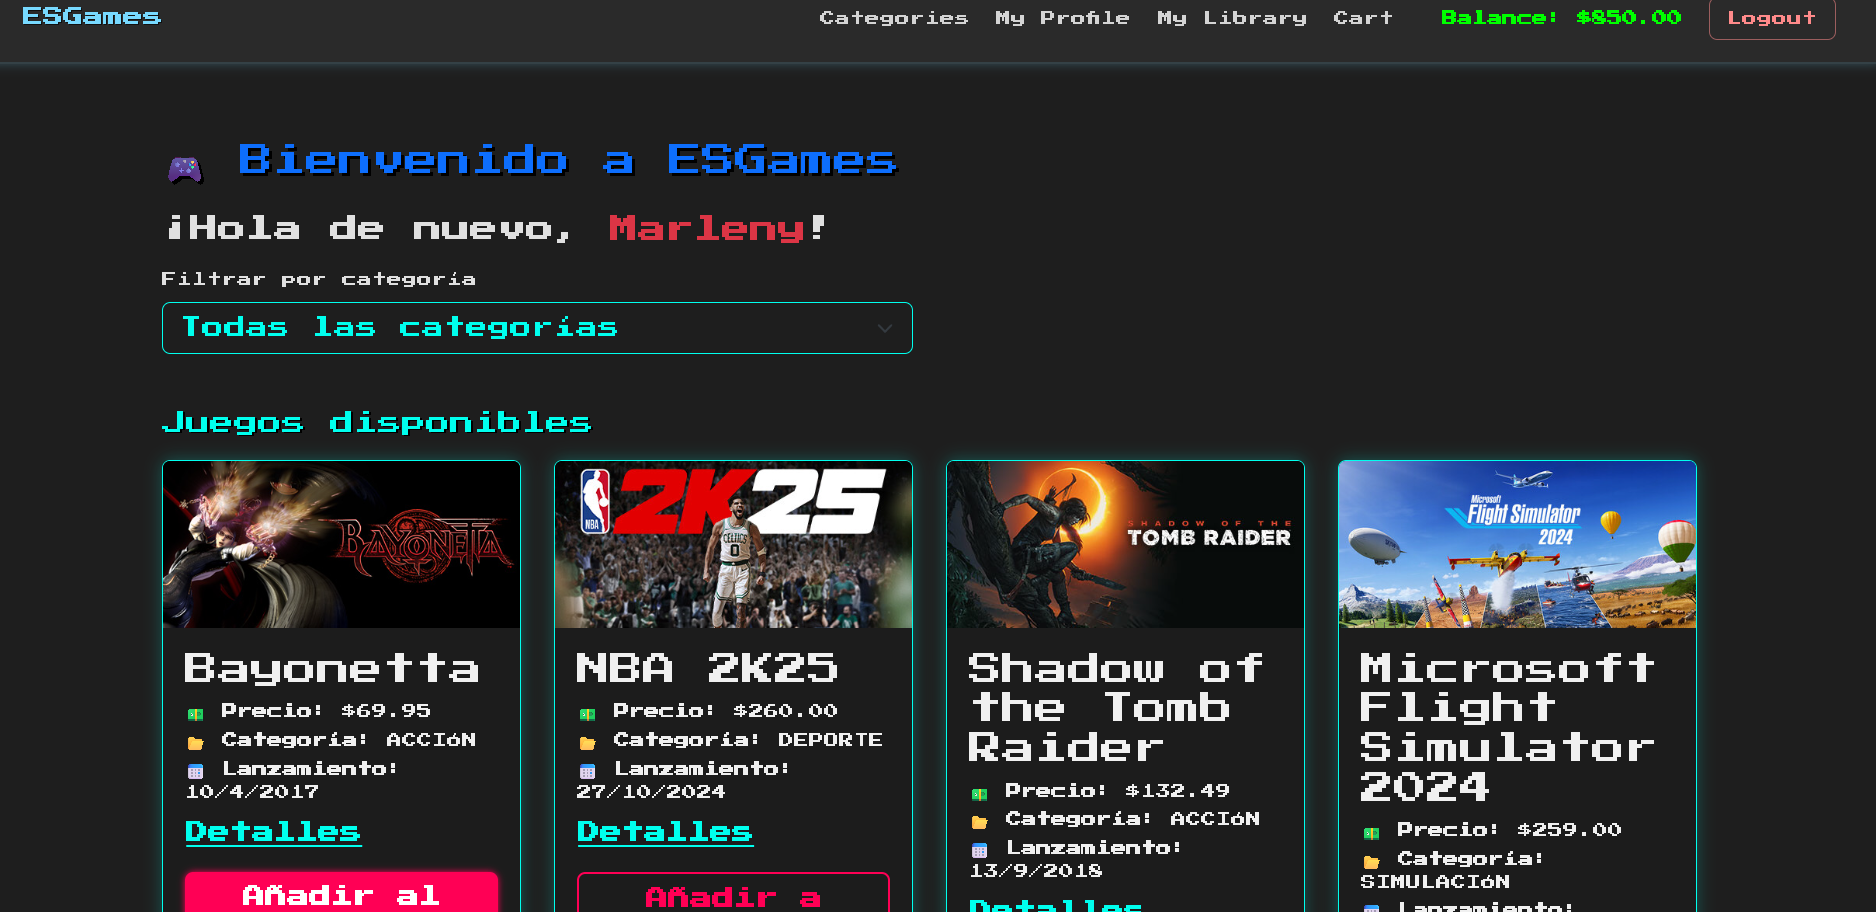
\includegraphics[width=0.9\linewidth]{img/webb.png}
    \caption{Interfas Principal con usuario registrado}
\end{figure}

\section{Servicios mediante una API RESTful}

El sistema \textbf{ESGames} expone su funcionalidad principal mediante una arquitectura RESTful, permitiendo la comunicación entre el frontend desarrollado en \texttt{Vue.js} y el backend en \texttt{Django}. Para la creación de esta API se utilizó el \texttt{Django REST Framework} (DRF), el cual facilita la serialización de datos, gestión de rutas, autenticación y validación de permisos.

\subsection{Estructura de la API}

Los recursos principales del sistema (usuarios, videojuegos, carrito, biblioteca, favoritos y reseñas) están expuestos a través de endpoints organizados bajo la estructura:

\begin{itemize}
    \item \texttt{/api/videogames/} \\
    Listado general de videojuegos disponibles. Soporta búsqueda y filtrado.

    \item \texttt{/api/cart/} \\
    Gestión del carrito de compras del usuario autenticado: agregar, actualizar o eliminar juegos.

    \item \texttt{/api/library/} \\
    Consulta de los videojuegos adquiridos por el usuario.

    \item \texttt{/api/reviews/} \\
    Lectura y creación de reseñas vinculadas a videojuegos comprados.

    \item \texttt{/api/favorites/} \\
    Agregado y eliminación de videojuegos marcados como favoritos.

    \item \texttt{/api/auth/} \\
    Módulo de autenticación: registro, login, obtención de token JWT.
\end{itemize}
\section{Seguridad y Autenticación con Tokens}

El sistema \textbf{ESGames} implementa un mecanismo de autenticación basado en \textit{tokens} para garantizar la seguridad de los recursos expuestos a través de su API RESTful. Esta técnica es fundamental para proteger las operaciones críticas, como la compra de videojuegos, la gestión del carrito, la visualización de bibliotecas personales y la publicación de reseñas.

\subsection{Autenticación Token}

El sistema utiliza el módulo \texttt{TokenAuthentication} de Django REST Framework para generar y validar tokens de sesión. Al momento del inicio de sesión, el servidor genera un token único para el usuario autenticado, el cual debe ser incluido en todas las solicitudes posteriores a endpoints protegidos.

\begin{verbatim}
POST /api/auth/login/
{
  "username": "usuario",
  "password": "clave123"
}
\end{verbatim}

La respuesta del servidor incluye el token:

\begin{verbatim}
{
  "token": "123abc456def..."
}
\end{verbatim}

Este token se almacena en el cliente (por ejemplo, en el \texttt{localStorage}) y se envía en el encabezado \texttt{Authorization} con cada solicitud autenticada:

\begin{verbatim}
Authorization: Token 123abc456def...
\end{verbatim}

\subsection{Protección de Endpoints}

Todos los endpoints sensibles (como la gestión de carrito, biblioteca, favoritos y reseñas) están protegidos mediante decoradores o clases que exigen autenticación previa. Por ejemplo:

\begin{verbatim}
from rest_framework.permissions import IsAuthenticated

class CartView(APIView):
    permission_classes = [IsAuthenticated]
    ...
\end{verbatim}

Esto garantiza que solo usuarios autenticados puedan acceder a recursos propios y realizar operaciones.

\subsection{Ventajas del Enfoque}

\begin{itemize}
    \item \textbf{Seguridad}: Los datos del usuario solo se exponen si el token válido es presentado.
    \item \textbf{Escalabilidad}: La autenticación por token permite integrar fácilmente otros clientes .
    \item \textbf{Independencia de Sesión}: A diferencia de las cookies, los tokens no dependen de sesiones almacenadas en el servidor.
\end{itemize}

\subsection{Buenas Prácticas Aplicadas}

\begin{itemize}
    \item Los tokens no se exponen en rutas públicas ni se almacenan en variables inseguras.
    \item Se recomienda usar HTTPS en producción para evitar ataques de tipo \textit{man-in-the-middle}.
\end{itemize}

Este sistema de autenticación proporciona una capa de seguridad robusta que protege los datos del usuario final y garantiza que las operaciones del sistema se ejecuten de manera segura.

\section{Servicios mediante una API RESTful}

El sistema \textbf{ESGames} expone su funcionalidad principal mediante una arquitectura RESTful, permitiendo la comunicación entre el frontend desarrollado en \texttt{Vue.js} y el backend en \texttt{Django}. Para la creación de esta API se utilizó el \texttt{Django REST Framework} (DRF), el cual facilita la serialización de datos, gestión de rutas, autenticación y validación de permisos.

\subsection{Estructura de la API}

Los recursos principales del sistema (usuarios, videojuegos, carrito, biblioteca, favoritos y reseñas) están expuestos a través de endpoints organizados bajo la estructura:

\begin{itemize}
    \item \texttt{/api/videogames/} \\
    Listado general de videojuegos disponibles. Soporta búsqueda y filtrado.

    \item \texttt{/api/cart/} \\
    Gestión del carrito de compras del usuario autenticado: agregar, actualizar o eliminar juegos.

    \item \texttt{/api/library/} \\
    Consulta de los videojuegos adquiridos por el usuario.

    \item \texttt{/api/reviews/} \\
    Lectura y creación de reseñas vinculadas a videojuegos comprados.

    \item \texttt{/api/favorites/} \\
    Agregado y eliminación de videojuegos marcados como favoritos.

    \item \texttt{/api/auth/} \\
    Módulo de autenticación: registro, login, obtención de token JWT.
\end{itemize}

\subsection{Serialización de Datos}

Cada modelo del sistema cuenta con su respectivo \texttt{serializer}, el cual transforma las instancias de objetos Python en datos JSON aptos para ser enviados al cliente. Por ejemplo, el modelo \texttt{Videogame} se serializa mediante:

\begin{verbatim}
class VideogameSerializer(serializers.ModelSerializer):
    class Meta:
        model = Videogame
        fields = '__all__'
\end{verbatim}

Estos serializadores también se encargan de validar datos de entrada antes de ser persistidos.

\subsection{Métodos HTTP y Operaciones}

La API expone los métodos HTTP estándares para operar sobre los recursos:

\begin{itemize}
    \item \texttt{GET}: Consultar información (ej. lista de juegos, detalles de un carrito, biblioteca del usuario).
    \item \texttt{POST}: Crear nuevos recursos (ej. agregar juegos al carrito, registrar un usuario, enviar una reseña).
    \item \texttt{PUT/PATCH}: Actualizar información existente (ej. cantidad de un juego en el carrito).
    \item \texttt{DELETE}: Eliminar elementos (ej. remover un juego de favoritos o del carrito).
\end{itemize}

\subsection{Consumo desde el Frontend}

Desde el cliente Vue.js, estas rutas se consumen mediante peticiones asincrónicas usando \texttt{fetch()} o librerías como \texttt{axios}. Por ejemplo:

\begin{verbatim}
const response = await fetch("https://api.esgames.com/api/videogames/");
const data = await response.json();
\end{verbatim}

Los datos se presentan dinámicamente en las vistas del sistema, con validaciones y retroalimentación para el usuario.

\subsection{Pruebas de Consumo}

Para verificar el correcto funcionamiento de la API, se realizaron pruebas desde distintas interfaces cliente:

\begin{itemize}
    \item Frontend oficial en Netlify.
    \item Herramientas de prueba como SoapUI.
\end{itemize}

Estas pruebas permitieron validar la consistencia de la API, la correcta autenticación y el cumplimiento del protocolo REST.
\section{Generación y Descarga de Boletas en PDF}

El sistema \textbf{ESGames} permite al usuario generar una boleta o comprobante digital al completar una compra. Esta funcionalidad tiene como propósito proporcionar al usuario un registro formal de su adquisición, incluyendo detalles como los videojuegos comprados, precios, fecha de transacción y datos personales del cliente.

\subsection{Renderización en HTML}

Inicialmente, la boleta es construida como una plantilla HTML estilizada, la cual se visualiza directamente desde el navegador luego de una compra exitosa. Esta plantilla utiliza etiquetas semánticas y estilos CSS definidos para garantizar una presentación clara, estructurada y adaptada al diseño general del sistema.

\subsection{Conversión a PDF}

Para permitir la descarga del comprobante, el HTML generado se convierte a formato PDF utilizando bibliotecas del entorno Python. En este caso, se empleó la librería \texttt{WeasyPrint}, la cual permite transformar contenido HTML + CSS a un documento PDF completamente formateado.

La conversión se realiza a través de una vista del backend, accesible mediante un endpoint autenticado:

\begin{verbatim}
from weasyprint import HTML
from django.http import HttpResponse

def generate_invoice_pdf(request, order_id):
    html_string = render_to_string("invoice_template.html", context)
    html = HTML(string=html_string)
    pdf = html.write_pdf()

    response = HttpResponse(pdf, content_type="application/pdf")
    response['Content-Disposition'] = 'attachment; filename="invoice.pdf"'
    return response
\end{verbatim}

\subsection{Descarga desde el Frontend}

En el frontend, el usuario puede descargar el comprobante haciendo clic en un botón disponible al finalizar su compra. Esta acción realiza una solicitud al endpoint correspondiente y fuerza la descarga del archivo:

\begin{verbatim}
<a :href="`/api/invoice/${orderId}/`" target="_blank">
    Descargar Boleta PDF
</a>
\end{verbatim}

\subsection{Contenido de la Boleta}

El PDF generado incluye la siguiente información:

\begin{itemize}
    \item Datos del cliente 
    \item Lista de videojuegos adquiridos
    \item Precios unitarios y subtotal
    \item Fecha y hora de la transacción
    \item Identificador de la operación
\end{itemize}

\subsection{Beneficios del Formato PDF}

\begin{itemize}
    \item \textbf{Portabilidad:} Los comprobantes pueden ser almacenados localmente por el usuario.
    \item \textbf{Impresión:} El formato PDF es apto para impresión sin pérdida de formato.
    \item \textbf{Validez documental:} Sirve como evidencia de compra para el usuario ante futuras consultas.
\end{itemize}

Esta funcionalidad añade una capa de profesionalismo y confianza en el proceso de compra, mejorando la experiencia del cliente final.


\section{Recursos en Línea}

A continuación, se presentan los enlaces oficiales relacionados con el proyecto \textbf{ESGames}, tanto del código fuente como del sistema desplegado para uso público.

\subsection{Repositorio del Proyecto}

El código fuente completo del sistema se encuentra disponible en la plataforma GitHub. Este repositorio contiene el backend desarrollado con Django, el frontend construido con Vue.js y Vite, así como documentación técnica complementaria.

\begin{itemize}
    \item \textbf{Repositorio GitHub:} \\
    \url{https://github.com/RodrigoFFN/Proyecto_Final_gameStore.git}
\end{itemize}

\subsection{Sitio Web en Producción}

El sistema se encuentra desplegado en línea para uso y evaluación a través del servicio \texttt{Netlify}, permitiendo a los usuarios interactuar con la tienda, registrarse, explorar videojuegos y simular compras reales.

\begin{itemize}
    \item \textbf{Enlace de acceso:} \\
    \url{https://esgamesproject.netlify.app/}
\end{itemize}

Ambos recursos permiten la validación funcional del sistema.
\section{Adicionales}

\subsection{Docentes Responsables del Curso}

Durante el desarrollo de este proyecto, el curso fue llevado en modalidad teórico–práctica, bajo la orientación de los siguientes docentes:

\begin{itemize}
    \item \textbf{Teoría:} Mg. Richart Smith Escobedo Quispe
    \item \textbf{Laboratorio:} Mg. Carlo José Luis Corrales Delgado
\end{itemize}

Ambos docentes brindaron las bases conceptuales y técnicas necesarias para el desarrollo de aplicaciones web modernas utilizando tecnologías actuales del backend y frontend.

\subsection{Autoevaluación}

A continuación, se presenta la imagen correspondiente a la autoevaluación del equipo con relación a su desempeño en el proyecto:

\begin{figure}[H]
    \centering
    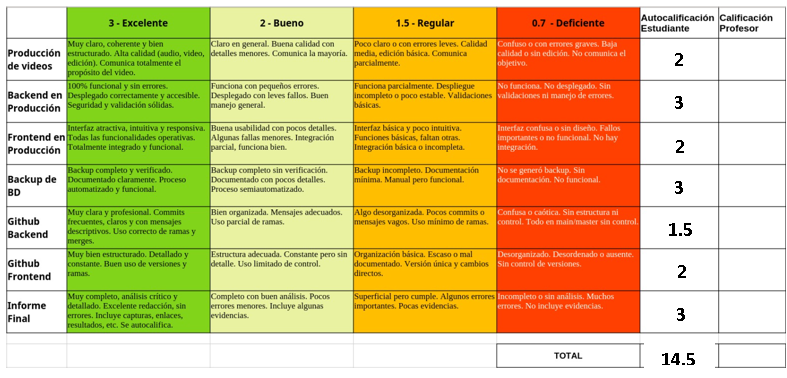
\includegraphics[width=0.65\textwidth]{img/autoevaluacion.png}
    \caption{Imagen de autoevaluación del estudiante}
\end{figure}


\section{Conclusiones}

El desarrollo del sistema \textbf{ESGames} ha permitido consolidar una solución web funcional e integral para la gestión de una tienda digital de videojuegos. A lo largo del proyecto, se logró implementar satisfactoriamente tanto el frontend como el backend, integrando múltiples tecnologías modernas que permiten una experiencia fluida, segura y modular para el usuario final.

Entre los principales logros del sistema se destacan:

\begin{itemize}
    \item La creación de una interfaz de usuario dinámica y responsiva utilizando \texttt{Vue.js}, desplegada eficientemente en \texttt{Netlify}.
    \item La implementación de una API RESTful robusta mediante \texttt{Django REST Framework}, con autenticación, control de acceso, validación de reglas de negocio y persistencia de datos.
    \item La integración con \texttt{Supabase} como sistema de base de datos relacional, y la utilización de \texttt{Render} para el despliegue del backend.
    \item La generación de boletas de compra en formato PDF, ofreciendo un respaldo formal a los usuarios por cada transacción realizada.
\end{itemize}

Asimismo, se destaca el valor que la aplicación entrega al usuario, permitiéndole explorar un catálogo de videojuegos, realizar compras simuladas, gestionar su biblioteca personal y dejar valoraciones útiles para otros compradores. Esto hace de ESGames una plataforma versátil y con potencial de crecimiento.

Como trabajo futuro se plantea:

\begin{itemize}
    \item Integrar pasarelas de pago reales.
    \item Añadir notificaciones por correo electrónico tras cada compra.
    \item Incorporar un sistema de roles para la administración y gestión del inventario.
    \item Ampliar el catálogo con funcionalidades de búsqueda avanzada y recomendaciones.
\end{itemize}

En conclusión, el proyecto ha cumplido los objetivos propuestos, ofreciendo una base sólida para una plataforma de e-commerce especializada en videojuegos, con miras a seguir evolucionando en futuras versiones.



\begin{thebibliography}{99}

\bibitem{django}
Django Software Foundation. (2024). \textit{Django Documentation (v4.x)}. Recuperado de \url{https://docs.djangoproject.com/}

\bibitem{drf}
Encode. (2024). \textit{Django REST Framework}. Recuperado de \url{https://www.django-rest-framework.org/}

\bibitem{vue}
Vue.js. (2024). \textit{Vue 3 Documentation}. Recuperado de \url{https://vuejs.org/}

\bibitem{vite}
Vite. (2024). \textit{Vite – Next Generation Frontend Tooling}. Recuperado de \url{https://vitejs.dev/}

\bibitem{netlify}
Netlify. (2024). \textit{Netlify Documentation}. Recuperado de \url{https://docs.netlify.com/}

\bibitem{render}
Render. (2024). \textit{Render Docs: Django Deployment}. Recuperado de \url{https://render.com/docs}

\bibitem{supabase}
Supabase. (2024). \textit{Supabase Documentation}. Recuperado de \url{https://supabase.com/docs}

\bibitem{weasyprint}
WeasyPrint. (2024). \textit{WeasyPrint Documentation}. Recuperado de \url{https://weasyprint.readthedocs.io/}

\bibitem{pinia}
Pinia. (2024). \textit{Pinia – Vue Store}. Recuperado de \url{https://pinia.vuejs.org/}

\bibitem{fetch}
Mozilla Developer Network (MDN). (2024). \textit{Fetch API}. Recuperado de \url{https://developer.mozilla.org/es/docs/Web/API/Fetch_API}

\end{thebibliography}

	
%\clearpage
%\bibliographystyle{apalike}
%\bibliographystyle{IEEEtranN}
%\bibliography{bibliography}
			
\end{document}